%++++++++++++++++++++++++++++++++++++++++
% Don't modify this section unless you know what you're doing!
\documentclass[a4paper,12pt]{article}
\usepackage{tabularx} % extra features for tabular environment
\usepackage{amsmath}  % improve math presentation
\usepackage{graphicx} % takes care of graphic including machinery
\usepackage[margin=0.8in,a4paper]{geometry} % decreases margins
\usepackage{cite} % takes care of citations
\usepackage[final]{hyperref} % adds hyper links inside the generated pdf file
\hypersetup{
	colorlinks=true,       % false: boxed links; true: colored links
	linkcolor=blue,        % color of internal links
	citecolor=blue,        % color of links to bibliography
	filecolor=magenta,     % color of file links
	urlcolor=blue         
}
%++++++++++++++++++++++++++++++++++++++++


\begin{document}

\title{Introduction to Compiler Construction 2016}
\author{Alexander Mayer, Daniel Schlager}
\date{\today}
\maketitle

\begin{abstract}
In this class we had to implement 11 features to extend the existing selfie-project\cite{cksystemsteaching}.
\end{abstract}

\newpage
\tableofcontents
\newpage

\section{Assignment 0}
Team: USEG\\
Members: Alexander Mayer, Daniel Schlager

\section{Assignment 1: Bitwise Shift Instructions}
In the first assignment we extended the mipster emulator, to support:
\begin{itemize}
\item sll
\item srl
\item sllv
\item slrv 
\end{itemize}
To do this, we had to change the existing opcode 0, which was used for the NOP instruction\cite{mips}. For the other three instructions, we did not have to change any existing code. As the shamt bits of the instructions in R format\cite{mips} was never used, we had to add a getShift function, which extracted the afore mentioned bits. This was necessary to decode the whole instruction properly.\\\\
$\Rightarrow$ This part works as expected in our implementation.

\section{Assignment 2: Bitwise Shift Operators (Scanning, Parsing)}
For the second assignment, we modified the scanner and added an additional layer in the parser. First, we extended the symbol table, so that the scanner would recognise the 
\begin{center}$<<$ and $>>$\end{center}
symbols. Next, we added the gr\_ShiftExpression to the parser. To take care of precedence, we put this procedure between gr\_expression and gr\_simpleExpression, as specified in the C standard\cite{cs50}.\\\\
$\Rightarrow$ This part is also working as expected.

\section{Assignment 3: Bitwise Shift Operators (Code Generation, Self-Compilation)}
To make assignment 3 work, we had to emit the code necessary for shifting in mipster. As the other parts were already taken care of in the first two assignments, self compilation already worked. We were able to replace the old implementation of shifts right away. \\\\
$\Rightarrow$ We did not encounter any problems here, everything is working. 
\newpage
\section{Assignment 4: Constant Folding} 
For constant folding, we generated an attribute (constantVal), which was used, whenever consant folding was possible. If a constant is found in a foldable position, we delay code generation by storing the mentioned constant in the constantVal attribute and passing it up to the next procedure to handle the code generation. Our compiler supports constant folding all the way up to gr\_expression. \\\\
$\Rightarrow$ This assignment also works as expected, however, we do not fold expressions like 
\begin{verbatim}
	x = 1 + x + 2;
\end{verbatim}
to avoid additional overhead.

\section{Assignment 5: Arrays}
To support arrays, we had to take care of declaration, as well as access of arrays. First, we added the bracket symbols $[$ and $]$ to the scanner. To allocate the right chunk of memory for an array, we added a size parameter to the symbol table entries.\\Memory for arrays is allocated on the stack, the first entry is starting at the lowest memory address, that is assigned to an array. When arrays are passed as parameters, they are stored at the very beginning of a frame. We just use 4 bytes to reference the actual array, the contents are not copied.\\The parameter therefore is just a pointer to the first entry of an array. In gr\_selector, we are generating the correct address. A differentiation is necessary, as an array, which is actually a parameter, has to dereference one more pointer to access the right address. For a regular access, we calculate the offset as follows: 
\begin{verbatim}
	a[i] = a + i * sizeoftype
\end{verbatim}
To make arrays work globally and locally, we had to modify gr\_factor, gr\_cstar, gr\_statement, gr\_procedure. Moreover, we had to introduce a new type called intarray\_t, in order to make the symbol table work correctly.\\\\
$\Rightarrow$ Arrays work as expected, but we do not support arrays for datastructures with types, that do not use 4 bytes per entry. 

\section{Assignment 6: Two-Dimensional Arrays}
For assignment 6, we had to extend the symbol table entries once more, we added the size of the second dimension, which is necessary to calculate the address that needs to be accessed correctly. \\The calculation for array access now looks as follows:
\begin{verbatim}
	a[i][j] = a + i * sizeofj * sizeoftype + j * sizeoftype
\end{verbatim}
This implies, that we are storing the dimention as follows:

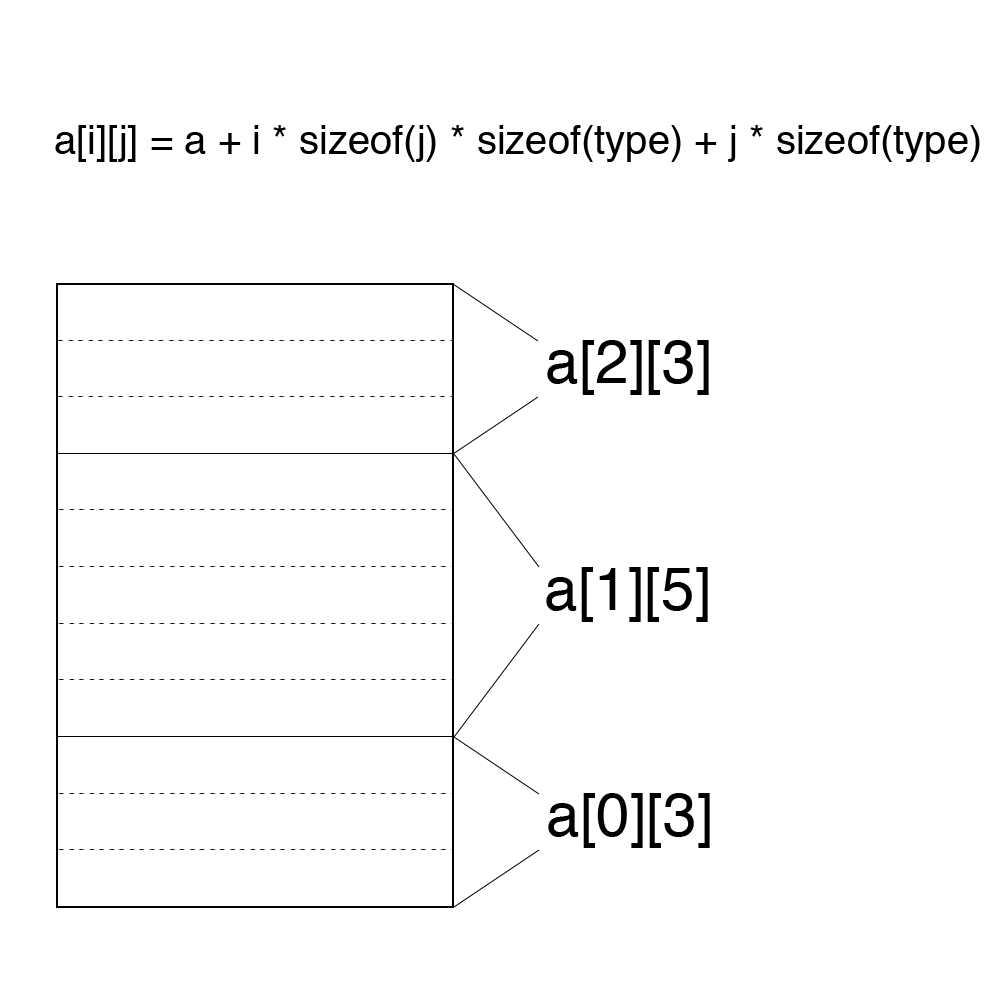
\includegraphics[scale=0.4]{array.png} 

$\Rightarrow$ Two dimensional arrays are working with the same restriction as one dimensional arrays.

\section{Assignment 7: Struct Declarations}
In assignment 7 we deviated from the C standard\cite{cs50} for the first time. When we declare a struct, it is internally handled like C's typedef struct. We generate a prototype in the global symbol table, but we do not allocate any memory. 
Members of structs are being stored in an extra struct table, which is referenced by the members parameter, that we added to the symbol table. We agreed on this implementation, because it is not necessary to add another class to selfie. Similar to the array assignment, we introduced a struct\_t type for the symbol table.\\As structs are allocated on the heap, we saved the relative offset of each member, in order to access members by name instead of index (this is the main difference between structs and arrays). Declaration of structs is handled in gr\_cstar and gr\_procedure.
\\\\
$\Rightarrow$ Struct declaration works without problems, it does however deviate from the C standard\cite{cs50}, as mentioned above. 

\section{Assignment 8: Struct Access}
For struct access, we introduced a procedure called gr\_struct, which checks the correct reference type and looks up the needed offset. This procedure is called by gr\_factor and gr\_statement. \\
\\\\
$\Rightarrow$ All our test cases worked for structs, we did not manage to implement symbol table entries as structs though, we did not find the bug. 

\section{Assignment 9: Boolean Operators (Individual)}
Boolean Operators are handled similarly to constant folding. Again, we used the attribute constantVal to pass up the fixup chains up for later handling. Everytime an \&\& or $||$ symbol gets detected by the parser, a branch instruction is being emitted, but since we do not know the final address of the jump, we have to do a fixup as soon as we know the correct offsets.\\These fixups make lazy evaluation, our goal, work. We implemented the \! operation, which flips the content of the current temporary. \\\\
$\Rightarrow$ There is a bug in our implementation of this feature, which we did not fix yet. We found the problem, and we will try to fix it as soon as time allows it. 

\section{Assignment 10: Boolean Operators (Algebra)}
Since \&\& and $||$ do not have the same precedence according to C standard\cite{cs50}, we implemented a new procedure called gr\_andExpression, that only deals with \&\& operations. $||$ is handled in gr\_expression now. This separation allows us to check for previous fixups, and deal with them accordingly. A merge of fixup chains, as discussed in class and out of class was not necessary to make our impementation work. \\\\
$\Rightarrow$ We did not stumble upon any errors here. 

\section{Assignment 11: Memory Management}
For our final assignment, we had to modify the malloc procedure as well as generate a free. The main thing to mind here is that we have to use storeVirtualMemory to construct the free list in the emulated memory instead of the memory of the emulator itself. If we would have emmitted this step, it would still work in selfie, but would not be managable on a bare iron machine. The freelist is implemented as a linked list, where the next free memory location is stored into the freed memory (again, inside of the emulator).\\We only need one pointer to make this work. Keep in mind that this only works for chunks of memory of a fixed size. Variable sizes could be implemented by managing multiple freelists or by storing the available size in memory as well. 
\\\\
$\Rightarrow$ Our memory management works as expected, no bugs here. 
\begin{thebibliography}{99}

\bibitem{cksystemsteaching}
C. Kirsch, \textit{Selfie Project},
\texttt{https://github.com/cksystemsteaching/CC-Summer-2016}

\bibitem{niklauswirth}
Niklaus Wirth, \textit{Grundlagen und Techniken des Compilerbaus},
\texttt{ISBN-13: 978-3486709513}

\bibitem{cs50}
CS50, Harvard, \textit{C Operator Precendence},
\texttt{https://cs50.harvard.edu/resources/\\cppreference.com/operator\_precedence.html}

\bibitem{mips}
Wikipedia, \textit{MIPS Instruction Set},
\texttt{https://en.wikipedia.org/wiki/MIPS\_instruction\_set}

\end{thebibliography}


\end{document}
